% !TeX root = main.tex

\section{同调群的同伦不变性}

\subsection{单纯逼近定理}

希望对拓扑空间 $ X, Y $, 若 $ X\cong Y $, 则有 $ H_p(X)\cong H_p(Y) $. 对可以三角剖分的拓扑空间, 存在复形 $ K $ 使得 $ X=\abs{K} $. 于是希望 $ \abs{K}\cong\abs{L} $ 时有 $ H_p(\abs{K})\cong H_p(\abs{L}) $. 一个自然的问题是如何定义 $ H_p(\abs{K}) $.

对任何 $ \abs{K} $ 的三角剖分 $ K',\ K'' $, 有 $ \abs{K'}=\abs{K''} $ 成立, 于是定义 $ H_p(\abs{K})=H_p(K) $ 即可.

考虑 $ f\in C(\abs{K},\abs{L}) $, 它未必是单纯映射. 我们希望找到单纯映射 $ g : K\to L $ 使得 $ \tilde{g} : \abs{K}\to\abs{L} $ 满足 $ f=\tilde{g} $, 即寻找一个单纯映射用来 ``代替'' $ f $.

\begin{Definition}[单纯逼近]
	设 $ f : C(\abs{K},\abs{L}) $, 称单纯映射 $ g $ 是 $ f $ 的\emph{单纯逼近}, 若对任意 $ x\in\abs{K} $ 都有
	\[
		\exists!\sigma\in K\,(x\in\mathrm{Int}\,\sigma)\land\exists\tau\in L\,(f(x)\in\mathrm{Int}\,\tau\land g(x)\in\tau).
	\]
	即 $ f(x) $ 与 $ g(x) $ 落在 $ L $ 的同一个单形 $ \tau $ 中.
\end{Definition}

\begin{Proposition}
	设 $ g $ 是 $ f\in C(\abs{K},\abs{L}) $ 的单纯逼近, 仍记它诱导的连续映射为 $ g $, 则 $ f\simeq g $. 更具体地, 若 $ f $ 可以被单纯映射诱导, 则 $ f=g $.
\end{Proposition}
\begin{Proof}
	由单纯映射的定义可知存在 $ \tau\in L $ 使得 $ f(x),g(x)\in\tau $, 而单形 $ \tau $ 是一个凸集. 于是总存在同伦
	\[
		H(x,t)=tf(x)+(1-t)g(x).
	\]
	任取 $ v\in K^{(0)} $, 因 $ f $ 被单纯映射诱导, 于是 $ f(v)\in L^{(0)} $. 而 $ g $ 是 $ f $ 的单纯逼近, 于是
	\[
		\forall v\in K^{(0)}\,(f(v)=w=g(v)\in L^{(0)}),
	\]
	这即 $ f|_{K^{(0)}}=g|_{K^{(0)}} : K^{(0)}\to L^{(0)} $. 进而 $ f=g $, 因从顶点出发可以一直诱导在高维骨架上的相等.\qed
\end{Proof}

然而并不是所有的连续映射都存在单纯逼近, 考虑下面的例子: 设 $ K $ 的几何实现为 $ \S^1 $, 而 $ L $ 的几何实现是一个平环 $ \set{z\in\C : 1\leqslant\abs{z}\leqslant 2} $.
\begin{figure}[htbp]
	\centering
	\includegraphics[width=0.5\linewidth]{figures/Sec5-1.png}
\end{figure}~\\
这因任何 $ K\to L $ 的单纯映射必定落在 $ L $ 的一个 2--单形中. 下面的问题就是: 在什么条件下存在单纯逼近?

\begin{Definition}[Star, Link]
	设 $ K $ 是一个复形, $ v\in K^{(0)} $, 定义
	\[
		\St(v,K)=\bigcup_{\sigma\in K,v\in\sigma}\mathrm{Int}\,\sigma,
	\]
	称作 $ v $ 在 $ K $ 中的 \emph{star}. 并记
	\[
		\mathrm{Link}\,(v,K):=\baro{\St(v,K)}\sm\St(v,K)=\bigcup_{v*\tau\in K}\tau,
	\]
	称作 $ v $ 在 $ K $ 中的 \emph{link}.
\end{Definition}

\begin{Proposition}
	$ \St(v,K) $ 是 $ \abs{K} $ 中的开集.
\end{Proposition}
\begin{Proof}
	这因
	\[
		\abs{K}\sm\St(v,K)=\bigcup_{\sigma\in K,v\notin\sigma}\sigma=L
	\]
	是 $ \abs{K} $ 中的闭子集, 其中 $ L=\set{\sigma\in K : v\notin\sigma} $ 是 $ K $ 的子复形.\qed
\end{Proof}

但 $ \mathrm{Int}\,\sigma $ 在一般的情况下未必是 $ \abs{K} $ 中的开集.
\begin{figure}[htbp]
	\centering
	\includegraphics[width=0.6\linewidth]{figures/Sec5-2.png}
	\caption{一个 $ \mathrm{Int}\,\sigma $ 不是 $ \abs{K} $ 中开集的例子}
\end{figure}~\\
而 link 就要更复杂一些, 下图给出了一个简单的2维复形中 link 的图示:
\begin{figure}[htbp]
	\centering
	\includegraphics[width=0.8\linewidth]{figures/Sec5-3.png}
	\caption{一个2维复形中顶点的闭Star, Star 和 Link}
\end{figure}

\begin{Proposition}\label{prop:5.5}
	设 $ \set{v_0,\dots,v_p}\subset K^{(0)} $, 则 $ \set{v_0,\dots,v_p} $ 落在某一单形中当且仅当 $ \bigcap_{i=0}^p\St(v_i,K)\ne\emptyset $.
\end{Proposition}
\begin{Proof}
	\textit{必要性.} 取 $ \sigma=(v_0,\dots,v_p)\in K^{(0)} $, 则 $ \forall i\in\set{0,\dots,p} $, 有
	\[
		\mathrm{Int}\,\sigma\subset\St(v_i,K)\Longrightarrow \mathrm{Int}\,\sigma\subset\bigcap_{i=0}^n\St(v_i,K),
	\]
	而 $ \mathrm{Int}\,\sigma\ne\emptyset $.

	\textit{充分性.} 取 $ x\in\bigcap_{i=0}^p\St(v_i,K)\subset \abs{K}=\bigcup_{\sigma\in K}\mathrm{Int}\,\sigma $. 则存在 $ \sigma\in K $ 使得 $ x\in\mathrm{Int}\,\sigma $. 由 star 的定义, $ v_i $ 是 $ \sigma $ 的顶点, 即 $ v_0,\dots,v_p $ 是 $ \sigma $ 中的顶点.\qed
\end{Proof}

\begin{Definition}[Star 条件]
	设映射 $ f\in C(\abs{K},\abs{L}) $, 称 $ f $ 满足 \emph{star 条件}, 若
	\[
		\forall v\in K^{(0)}\,\exists w\in L^{(0)}\,(f(\St(v,K))\subset\St(w,L)).
	\]
\end{Definition}

\begin{Proposition}[用 star 条件刻画单纯逼近]
	$ f\in C(\abs{K},\abs{L}) $ 存在单纯逼近当且仅当它满足 star 条件. 特别地, 若 $ g $ 是 $ f $ 的单纯逼近, 则对任意 $ v\in K^{(0)} $, 有
	\[
		f(\St(v,K))\subset\St(g(v),L).
	\]
\end{Proposition}
\begin{Proof}
	\textit{必要性.} 设 $ g : K\to L $ 是 $ f $ 的单纯逼近, 只需证明
	\[
		\forall v\in K^{(0)}\,(f(\St(v,K))\subset\St(g(v),L)).
	\]
	
	任取 $ x\in\St(v,K) $, 根据 star 的定义可知存在 $ \sigma\in K $ 使得 $ x\in\mathrm{Int}\,\sigma $ 且 $ v\in\sigma $. 又因为 $ g $ 是 $ f $ 的单纯逼近, 故存在 $ \tau\in L $ 使得 $ f(x)\in\mathrm{Int}\,\tau $ 且 $ g(x)\in\tau $. 因 $ g $ 是单纯映射, $ g(\sigma)=\tau_1\in L $, 且 $ g(v)\in g(\sigma) $. 断言 $ g(x)\in\mathrm{Int}\,\tau_1 $. 注意到对 $ \sigma=(v_0,\dots,v_p) $,
	\[
		x=\sum_{i=0}^pt_iv_i\Longrightarrow g(x)=\sum_{i=0}^pt_ig(v_i)\in\mathrm{Int}\,\tau_1,
	\]
	(\textit{即使 $ g(v_i) $ 中有相等项也没有关系}), 于是断言成立. 因 $ g(x)\in\tau $, 故 $ \tau_1\subset\tau $. 而 $ g(v) $ 是 $ \tau_1 $ 的顶点, 故它也是 $ \tau $ 的顶点.

	此时, $ f(x)\in\mathrm{Int}\,\tau\subset\St(g(v),L) $, 也即 $ f(\St(v,K))\subset\St(g(v),L) $.

	\textit{充分性.} 假设 $ f $ 满足 star 条件, 由这一条件可以定义映射 $ g $
	\[
		g : K^{(0)}\to L^{(0)},\qquad v\mapsto g(v)=w
	\]
	使得 $ f(\St(v,K))\subset\St(g(v),L) $. 下面将 $ g $ 扩张成一个单纯映射.

	任取 $ \sigma=(v_0,\dots,v_p)\in K $, 只需证明 $ \set{g(v_0),\dots,g(v_p)} $ 落在 $ L $ 的同一单形中. 由~\ref{prop:5.5}~知 $ \bigcap_{i=0}^p\St(v_i,K)\ne\emptyset $. 故
	\[
		\emptyset\ne f\left( \bigcap_{i=0}^p\St(v_i,K) \right)\subset\bigcap_{i=0}^pf(\St(v_i,K))\subset\bigcap_{i=0}^p\St(g(v_i),L).
	\]
	再由~\ref{prop:5.5}~可知 $ \set{g(v_0),\dots,g(v_p)} $ 落在 $ L $ 的某一单形中, 不妨记作 $ \tau=:g(\sigma) $, 故 $ g $ 是单纯映射.

	再证 $ g $ 是 $ f $ 的单纯逼近, 首先
	\[
		\forall x\in\abs{K}=\bigcup_{\sigma\in K}\mathrm{Int}\,\sigma\,\exists!\sigma=(v_0,\dots,v_p)\in K\,\forall i\,(x\in\mathrm{Int}\,\sigma\subset\St(v_i,K)).
	\]
	由题设和 star 的定义, 因 $ f(x)\in\St(g(v_i),L) $, 有
	\[
		\exists\tau\in L\,(f(x)\in\mathrm{Int}\,\tau),
	\]
	此时可知 $ g(v_i)\in\tau $. 对 $ x=\sum_{i=0}^pt_iv_i $, 都有 $ g(x)=\sum_{i=0}^pt_ig(v_i)\in\tau $. 故 $ g $ 是 $ f $ 的一个单纯逼近.\qed
\end{Proof}

单纯逼近不能解决所有问题, 例如之前的例子
\begin{figure}[htbp]
	\centering
	\includegraphics[width=0.5\linewidth]{figures/Sec5-1.png}
\end{figure}
中 $ f $ 不存在单纯逼近. 此时就需要另外一种工具: 重分.

\begin{Definition}[重分]
	称 $ K' $ 是 $ K $ 的一个\emph{重分}, 若
	\begin{enumerate}[(1)]
		\item $ \forall\tau\in K'\,\exists\sigma\in K\,(\tau\subset\sigma) $, 即重分只能分出更小的单形.
		\item $ \forall\sigma\in K\,\exists\tau_1,\dots,\tau_r\in K'\,(\sigma=\bigcup_{i=1}^r\tau_i) $, 即重分都是有限分割.
	\end{enumerate}
	注意到在 $ \R^\N $ 中 $ \abs{K'}=\abs{K} $, 于是重分实际上只是将 star 变小了.
\end{Definition}

\begin{Theorem}[单纯逼近定理]\label{thm:单纯逼近定理}
	对任意的 $ f\in C(\abs{K},\abs{L}) $, 存在 $ K $ 的重分 $ K' $ 使得 $ f\in C(\abs{K'},\abs{L}) $ 存在单纯逼近 $ g : K'\to L $.
\end{Theorem}

这是本节的中心定理, 我们只处理 $ K $ 是有限复形的情形. 但即使如此, 我们也需要先进行以下的准备工作, 再回来处理这一定理的证明.

\begin{Lemma}
	任取 $ w\in K^{(0)} $, 存在 $ v\in K $ 使得 $ \St(w,K)\subset\St(v,K) $.
\end{Lemma}

\begin{Proposition}
	$ \id : \abs{K'}\to\abs{K} $ 存在单纯逼近 $ g : K'\to K $.
\end{Proposition}

\begin{Definition}[标准重心重分]
	对 $ \sigma=(v_0,\dots,v_p) $, 其\emph{重心}定义为
	\[
		\hat{\sigma}=\frac{v_0+\dots+v_p}{p+1}.
	\]
	归纳地定义: $ p=0 $ 时, 在 $ K^{(0)} $ 上 $ L^{(0)}=K^{(0)} $; $ p=1 $ 时, 在 $ K^{(1)} $ 上
	\[
		L^{(1)}=\set{\hat{\sigma}*L_\sigma : \sigma\in K^{(1)},\,\dim\sigma=1,\,\abs{L_\sigma}=\abs{\Bd\sigma}},
	\]
	归纳地, 当 $ p=k+1 $ 时, 在 $ K^{(k+1)} $ 上
	\[
		L^{(k+1)}:=\set{\hat{\sigma}*L_\sigma : \sigma\in K^{(k+1)},\,\dim\sigma=k+1,\,L_\sigma\subset L^{(k)}\,(\abs{L_\sigma}=\abs{\Bd\sigma})},
	\]
	并称 $ \sd\,K=\bigcup_{p\geqslant 0}L^{(p)} $ 为 $ K $ 的\emph{标准重心重分}. 类似地记 $ \sd^2=\sd(\sd\,K) $.

	\begin{figure}[htbp]
		\centering
		\includegraphics[width=0.4\linewidth]{figures/Sec5-4.png}
		\caption{一个2维单形构成的复形及其标准重心重分}
	\end{figure}

	也可以这样定义标准重心重分:
	
	称 $ K $ 中的一列 $ \sigma_1\subset\sigma_2\subset\dots\subset\sigma_r $ 是一个 \emph{flag}, 它确定单形 $ (\hat{\sigma}_1,\dots,\hat{\sigma}_r) $(\textit{注意到它也可以唯一地确定 flag}), 定义
	\[
		\sd\,K:=\set{(\hat{\sigma}_1,\dots,\hat{\sigma}_r) : \sigma_1\subset\dots\subset\sigma_r}=\set{\sigma_1\subset\dots\subset\sigma_r}.
	\]
\end{Definition}

\begin{Definition}[网径]
	当 $ K $ 是有限复形时, 定义 $ K $ 的\emph{网径}为
	\[
		\mesh K:=\max_{\sigma\in K}\diam\sigma=\max_{\sigma\in K}\max_{x,y\in\sigma}\norm{x-y}.
	\]
	那么 star 自然就有这样的性质: 对任意 $ v\in K^{(0)} $ 有 $ \St(v,K)\subset B(v,\mesh K) $.
\end{Definition}

直观上, 标准重心重分减小了网径, 即 $ \mesh\sd\,K<\mesh K $, 下面的引理给出了这一结论的一个估计:

\begin{Lemma}\label{lem:标准重心重分与网径}
	设 $ K $ 是有限复形, 则
	\[
		\mesh(\sd\,K)\leqslant\frac{n}{n+1}\mesh K,
	\]
	进而 $ m\to\infty $ 时 $ \mesh(\sd^m K)\to 0 $.
\end{Lemma}
\begin{Proof}
	对 $ \sigma=(v_0,\dots,v_p)\in K $, 有 $ \diam\sigma=\max_{i,j}\norm{v_i-v_j} $. 这因 $ \forall x,y\in\sigma $, 记 $ y=\sum_{i=0}^pt_iv_i $ 后
	\[
		\norm{x-y}\leqslant\norm{x-\sum_{i=0}^pt_iv_i}=\norm{\sum_{i=0}^pt_i(x-v_i)}\leqslant\max_{i}\norm{x-v_i},
	\]
	类似地 $ \norm{v_i-x}\leqslant\max_j\norm{v_i-v_j} $.

	任取 $ \tau,\sigma\in\sd\,K $, $ \tau\subset\sigma $. 则 $ \tau\subset\sigma\in K $. 设 $ \sigma=(v_0,\dots,v_p) $, 则存在 $ i_0\in\set{0,\dots,p} $ 使得
	\[
		\norm{\hat{\sigma}-\hat{\tau}}\leqslant\norm{\hat{\sigma}-v_{i_0}}=\norm{\frac{1}{p+1}\sum_{i-0}^pv_i-v_{i_0}}=\norm{\sum_{i=0}^p\frac{v_i-v_{i_0}}{p+1}}\leqslant\frac{p}{p+1}\mesh K.
	\]
	而 $ p\leqslant n $ 时总有 $ p/(p+1)\leqslant n/(n+1) $. 得证.\qed
\end{Proof}

现在我们回到单纯逼近定理~\ref{thm:单纯逼近定理}~的证明:

\textbf{定理~\ref{thm:单纯逼近定理}~的证明}\hspace{2\ccwd} 若 $ K $ 是有限复形, 则 $ \abs{K} $ 一定是紧度量空间. 由 Lebesgue 覆盖引理可知对任何开覆盖 $ \CA $, 都存在 Lebesgue 数 $ \delta>0 $ 使得
\[
	\forall x\in\abs{K}\,\exists C\in\CA\,(B(x,\delta)\subset C).
\]
对 $ f : \abs{K}\to\abs{L} $, 考虑 $ \abs{L} $ 的开覆盖 $ \set{\St(w,L) : w\in L^{(0)}} $, 存在 $ K $ 的开覆盖
\[
	\CA=\set{f^{-1}(\St(w,L)) : w\in L^{(0)}},
\]
由 Lebesgue 覆盖引理, 存在 $ \delta>0 $ 使得
\[
	\forall x\in\abs{K}\,\exists w\in L^{(0)}\,(B(x,\delta)\subset f^{-1}(\St(w,L))).
\]
由~\ref{lem:标准重心重分与网径}~可知存在正整数 $ m $ 使得 $ \mu=\mesh(\sd^m\,K)<\delta $. 任取 $ v\in(\sd^m\,K)^{(0)} $, 存在 $ w\in L^{(0)} $ 使得
\[
	\St(v,\sd^m\,K)\subset B(v,\mu)\subset B(v,\delta)\subset f^{-1}(\St(w,L)).
\]
也即 $ f(\St(v,\sd^m\,K))\subset\St(w,L) $. 这即 star 条件, 于是 $ f $ 存在单纯逼近 $ \varphi : \sd^m\,K\to L $.\qed

\subsection{链同伦}

在上一小节我们知道了对复形进行适当次数的标准重心重分, 就可以得到连续映射的单纯逼近. 还有两个问题需要考虑: 其一是\textit{不同的单纯逼近是否诱导相同的同态}; 其二是\textit{对不同的重分 $ K',\ K'' $ , 他们的同调群 $ H_p(K') $ 和 $ H_p(K'') $ 之间是否存在同态}.

本小节主要来讨论第一个问题:

\begin{Definition}[链同伦]
	设 $ \psi\,\psi' : C_p(K)\to C_p(L) $ 是链映射, 称 $ \psi $ 与 $ \psi' $ \emph{链同伦}, 若
	\[
		\exists D : C_p(K)\to C_{p+1}(L)\,(\partial D+D\partial=\psi-\psi'),
	\]
	记作 $ \psi\simeq\psi' $.
\end{Definition}

或者使用交换图的语言, 即图
\begin{center}
	\begin{tikzcd}
		& 	C_{p+1}(L) \arrow[d, "\partial"] \\
			C_p(K) \arrow[r] \arrow[r, "{\psi,\psi'}"] \arrow[ru, "D"] \arrow[d, "\partial"'] & C_p(L)                           \\
			C_{p-1}(K) \arrow[ru, "D"]                                                        &                                 
	\end{tikzcd}
\end{center}
交换.

\begin{Theorem}\label{thm:单纯逼近链同伦}
	设 $ \varphi,\ \varphi' : K\to L $ 都是 $ f : \abs{K}\to\abs{L} $ 的单纯逼近, 则 $ \varphi_\sharp\simeq\varphi_\sharp' $.
\end{Theorem}
\begin{Proof}
	任取 $ v\in K'^{(0)} $, $ \varphi,\ \varphi' $ 是 $ f $ 的单纯逼近, 故应当满足 star 条件
	\[
		f(\St(v,K')\subset\St(\varphi(v),L)\cap\St(\varphi'(v),L).
	\]
	对任意 $ x\in K $, 存在单形 $ \sigma=(v_0,\dots,v_p)\in K' $ 使得 $ x\in\mathrm{Int}\,\sigma $. 则存在 $ \tau\in L $ 使得
	\[
		f(x)\in\mathrm{Int}\,\tau,\qquad \varphi(x),\varphi'(x)\in\tau.
	\]
	对任意 $ i\in\set{0,\dots,p} $, 都有
	\[
		f(x)\in\mathrm{Int}\,\tau\subset f(\St(v_i),K)\subset\St(\varphi(v_i),L)\cap\St(\varphi'(v_i),L),
	\]
	故 $ \set{\varphi(v_0),\dots,\varphi(v_p),\varphi'(v_0),\dots,\varphi'(v_p)} $ 落在 $ L $ 的同一个单形中. 不妨记以这些顶点为顶点集生成的单形及其面构成的子复形为 $ L(\sigma) $. 则
	\[
		\dim L(\sigma)\leqslant 2p+1,
	\]
	且满足 $ L(\sigma) $ 非空, $ L(\sigma) $ 零调(\textit{这因 $ L(\sigma) $ 是单形生成的子复形}), 而且对 $ s\subset\sigma $, 有 $ L(s)\subset L(\sigma) $ (\textit{这只需注意到 $ L(s)^{(0)}\subset L(\sigma)^{(0)} $}). $ \varphi_\sharp(\sigma) $ 和 $ \varphi_\sharp'(\sigma) $ 被 $ L(\sigma) $ 承载.

	(\textit{下面这一段证明的 pattern 非常重要, 这是一类基本技巧, 请务必掌握.}) 归纳地证明结论: 当 $ p=0 $ 时, 对 $ v\in K^{(0)} $. 因 $ \varphi_\sharp(v)=\varphi(v) $, $ \varphi'_\sharp(v)=\varphi'(v) $, 于是自然有
	\[
		\varphi_\sharp(v),\varphi'_\sharp(v)\in C_0(L(v)).
	\]
	因 $ L(v) $ 道路连通, 故 $ \varphi_\sharp(v) $ 与 $ \varphi_\sharp'(v) $ 在同一同调类中, 考虑到 $ L(v) $ 零调, 于是
	\[
		\exists d\in C_1(L(v))\,(\partial d)=\varphi_\sharp(v)-\varphi'_\sharp(v),
	\]
	取 $ D(v)=d $ 即可. 此时
	\[
		\partial D_0(v)+D_{-1}\partial v=\partial D(c)=\varphi_{\sharp}(v)-\varphi'_\sharp(v)
	\]
	满足条件.

	接下来设对任意 $ <p-1 $ 的情形都成立, 那么对 $ p $ 的情形, 取 $ \sigma\in K' $, $ \dim\sigma=p $, 我们希望
	\[
		\partial D\sigma=\varphi_\sharp(\sigma)-\varphi'_\sharp(\sigma)-D\partial\sigma
	\]
	成立, 右侧的每一项都是已经定义过的, 记右侧为 $ c $, 计算
	\[
		\begin{aligned}
			\partial c&=\partial\varphi_\sharp(\sigma)-\partial\varphi'_\sharp(\sigma)-\partial D(\partial\sigma)\\
			&=\partial\varphi_\sharp(\sigma)-\partial\varphi'_\sharp(\sigma)-(\varphi_\sharp(\partial\sigma)-\varphi'_\sharp(\partial\sigma)-D\partial^2\sigma)\\
			&=0,
		\end{aligned}
	\]
	这因 $ \varphi_\sharp $ 和 $ \varphi_\sharp' $ 可以与 $ \partial $ 交换. 这说明 $ \set{c}\in H_p(L(\sigma)) $, 进一步 $ c $ 被 $ L(\sigma) $ 承载(\textit{因每一项都被 $ L(\sigma) $ 承载}). 故 $ \set{c}\in H_p(L(\sigma))=0 $, 也即 $ c\in Z_p(L(\sigma))=B_p(L(\sigma)) $, 于是
	\[
		\exists d\in C_{p+1}(L(\sigma))\,(\partial d=c),
	\]
	取 $ D(\sigma)=d $ 即可.

	由此, 我们归纳地构造了 $ D $ 满足链同伦的条件, 从而 $ \varphi_\sharp\simeq\varphi_\sharp' $.\qed
\end{Proof}

\begin{Corollary}
	设 $ \varphi,\ \varphi' : K\to L $ 都是 $ f : \abs{K}\to\abs{L} $ 的单纯逼近, 则 $ \varphi_*=\varphi'_* $.
\end{Corollary}
\begin{Proof}
	因对任意 $ z_p+B_p(K')\in H_p(K') $, 都有
	\[
		\begin{aligned}
			\varphi_*(z_p+B_p(K'))&=\varphi_*(z_p)+B_p(L)\\
			&=\partial D(z_p)+D(\partial z_p)+\varphi_*'(z_p)+B_p(L)\\
			&=\varphi_*'(z_p)+\partial D(z_p)+B_p(L)\\
			&=\varphi'_*(z_p)+B_p(L).
		\end{aligned}
	\]
	成立. 其中第二行的等号因 $ \partial z_p=0 $, 第三行的等号因 $ D(z_p)\in B_{p+1}(L) $ 导出 $ \partial D(z_p)\in B_p(L) $.\qed
\end{Proof}

\subsection{代数重分定理}

本小节主要来讨论第二个问题: 即单纯逼近导出的同态是否依赖于对复形 $ K $ 的重分. 设 $ K' $ 是 $ K $ 的重分, $ \id : \abs{K'}\to \abs{K} $ 有单纯逼近 $ g : K'\to K $. 那么 $ g $ 诱导的 $ g_* $ 是否是同构?
\begin{center}
	\begin{tikzcd}
		H_p(K)                                                       & H_p(L) \\
		H_p(K') \arrow[u, "g_*"] \arrow[ru, "\varphi_*=\varphi_*'"'] &       
		\end{tikzcd}
\end{center}
如果 $ g_* $ 是同构, 那么 $ H_p(K) $ 到 $ H_p(L) $ 的同态就可以给出.

为此考虑这样的一类映射:

\begin{Definition}[零调承载子]
	称 $ \varPhi : K\to L,\ \sigma\mapsto \varPhi(\sigma)\ne\emptyset $ 是一个\emph{零调承载子}, 若对任意 $ \sigma\in K $, 都有 $ \varPhi(\sigma) $ 零调. 且
	\[
		s\subset\sigma\Longrightarrow\varPhi(s)\subset\varPhi(\sigma).
	\]

	设 $ f : C_p(K)\to C_p(L) $ 是一个链映射, 称 $ f $ 被 $ \varPhi $ 承载, 若对任意 $ \sigma\in K $, $ \dim\sigma=p $ 都有 $ f(\sigma) $ 被 $ \varPhi(\sigma) $ 承载.
\end{Definition}

\begin{Proposition}[零调承载子定理]\label{prop:零调承载子定理}
	设 $ \varPhi : K\to L $ 是零调承载子:
	\begin{enumerate}
		\item 若 $ \varphi,\psi : \CC(K)\to\CC(L) $ 被 $ \varPhi $ 承载, 则存在 $ D $ 确定 $ \varphi\simeq\psi $;
		\item 存在被 $ \varPhi $ 承载的保持增广的链映射 $ \varphi : \CC(K)\to \CC(L) $.
	\end{enumerate}
\end{Proposition}
\begin{Proof}
	(1) 无非就是~\ref{thm:单纯逼近链同伦}~中使用相同的 pattern 证明, 只需要注意到 $ \varPhi(\sigma) $ 也满足相应的条件(\textit{非空, 零调, 保持包含}).

	(2) 归纳地, 
	\begin{center}
		\begin{tikzcd}
			{} \arrow[r] & C_p(K) \arrow[r] & \cdots \arrow[r] & C_1(K) \arrow[r, "\partial"] \arrow[dd, "\varphi_1"] \arrow[rdd, "\varphi_0\partial"', bend left] & C_0(K) \arrow[rd, "\varepsilon"] \arrow[dd, "\varphi_0"] &              &   \\
						 &                  &                  &                                                                                                   &                                                          & \Z \arrow[r] & 0 \\
			{} \arrow[r] & C_p(L) \arrow[r] & \cdots \arrow[r] & C_1(L) \arrow[r, "\partial"]                                                                      & C_0(L) \arrow[ru, "\varepsilon'"']                       &              &  
		\end{tikzcd}
	\end{center}
	当 $ p=0 $ 时, 取 $ v\in K^{(0)} $, $ \varepsilon(v)=1 $. 取 $ w $ 是 $ \varPhi(v) $ 的顶点, 并取 $ \varphi_0(v)=w $. 则
	\[
		1=\varepsilon(v)=\varepsilon'(\varphi(v))=\varepsilon'(w)=1,
	\]
	成立.

	当 $ p=1 $ 时, 取 $ \sigma=[v_0,v_1] $, $ \dim\sigma=1 $. 再取 $ c=\varphi_0(\partial\sigma) $, 那么
	\[
		\varepsilon'c=\varepsilon'\varphi_0(\partial\sigma)=\varepsilon(\partial\sigma)=0,
	\]
	即 $ c $ 是增广链中的闭链. 故 $ \set{c}\in\tilde{H}_0(\varPhi(\sigma))=0 $, 从而
	\[
		c\in\ker\varepsilon'=\im\partial\Longrightarrow\exists d\in C_1(\varPhi(\sigma))\subset C_1(L)\,(\partial d=c).
	\]
	定义 $ \varphi_1(\sigma)=d $ 即可. 由
	\[
		\partial\varphi_1(\sigma)=\partial d=\varphi_0(\partial\sigma)
	\]
	可知图中 $ C_1(K), C_0(K), C_1(L), C_0(L) $ 所在的方块交换.

	设 $ <p-1 $ 的情形都成立, 即对 $ \sigma\in K $, $ \dim\sigma<p-1 $ 都存在相应的 $ \varphi $ 被 $ \varPhi $ 承载. 取 $ \sigma\in K $, $ \dim\sigma=p $, 那么考虑
	\[
		\partial\varphi(\partial\sigma)=\varphi\partial^2\sigma=0,
	\]
	则
	\[
		\varphi(\partial\sigma)\in Z_p(\varPhi(\sigma))=B_p(\varPhi(\sigma))\Longrightarrow\exists d\in C_{p+1}(\varPhi(\sigma))\subset C_{p+1}(L)\,(\partial d=\varphi(\partial\sigma)).
	\]
	定义 $ \varphi(\sigma)=d $ 即可.
	
	至此, 我们归纳地构造了 $ \varphi $.\qed
\end{Proof}

现在提出本小节的中心定理: 

\begin{Theorem}[代数重分定理]\label{thm:代数重分定理}
	设 $ K' $ 是 $ K $ 的一个重分, 则
	\begin{enumerate}[(1)]
		\item 存在唯一的链映射 $ \lambda : C_p(K)\to C_p(K') $ 使得 $ \lambda(\sigma) $ 可被 $ K_\sigma' $ 承载, 称 $ \lambda $ 是\emph{重分算子}.
		\item $ \lambda $ 与 $ g_\sharp $ 互为链同伦逆, 由此 $ g_* $ 和 $ \lambda_* $ 均为同构.
	\end{enumerate}
\end{Theorem}
\begin{Proof}
	考虑
	\[
		\Lambda : K\to K',\qquad\sigma\mapsto\Lambda(\sigma)=K_\sigma',
	\]
	假设 $ K_\sigma' $ 是零调的. 此时 $ \Lambda $ 是零调承载子, 由~\ref{prop:零调承载子定理}~可知存在唯一的 $ \lambda $ 使得 $ \lambda(\sigma)\in\CC(\Lambda(\sigma)) $ 对任意 $ \sigma\in K $ 成立. 再考虑
	\[
		\Theta : K'\to K,\qquad \tau\mapsto\Theta(\tau)=K_{\sigma_\tau},
	\]
	其中 $ \sigma_\tau\in K $ 是包含 $ \tau $ 的最低维子复形. 故 $ K_{\sigma_\tau} $ 也是锥, 而锥是零调的. 此时 $ \Theta $ 也是零调承载子, 由~\ref{prop:零调承载子定理}~可知存在唯一的 $ \theta $ 使得 $ \theta(\tau)\in\CC(\Theta(\tau)) $ 对任意 $ \tau\in K' $ 成立.

	\begin{figure}[htbp]
		\centering
		\includegraphics[width=0.85\linewidth]{figures/Sec5-5.png}
	\end{figure}
	
	同样地, 可以得到 $ \id_{\CC(K)} $ 被 $ \Psi $ 承载, $ \id_{\CC(K')} $ 被 $ \varPhi $ 承载.

	\textbf{Claim 1.}\ \ $ \theta\circ\lambda : \CC(K)\to\CC(K) $ 被 $ \Psi $ 承载, $ \lambda\circ\theta : \CC(K')\to\CC(K') $ 被 $ \varPhi $ 承载.

	下面证明 Claim 1. 我们只说明 $ \theta\circ\lambda $ 被 $ \Psi $ 承载, 另一侧类似可证. 任取 $ \sigma\in K $, 由 $ \lambda(\sigma) $ 被 $ \Lambda(\sigma) $ 承载可知 $ \lambda(\sigma) $ 可以被 $ \Lambda(\sigma)=K_\sigma' $ 中单形 $ \tau<\sigma $ 线性表示. 又由 $ \theta(\tau) $ 被 $ \Theta(\tau) $ 承载可知 $ \Theta(\tau)=K_{\sigma_\tau}=K_\sigma=\Psi(\sigma) $. 由此 $ \theta\circ\lambda(\sigma) $ 可被 $ \Psi(\sigma)=K_\sigma $ 承载.

	\textbf{Claim 2.}\ \ $ \Theta $ 承载 $ g_\sharp $.

	下面证明 Claim 2. 任取 $ \tau\in K' $, $ w\in\tau $ 是其一个顶点. 由单纯逼近的 star 条件可知
	\[
		\mathrm{Int}\,\tau\subset\id(\St(w,K))\subset\St(g(w),K),
	\]
	设 $ \sigma $ 是顶点集含有 $ g(w) $ 的单形, 则 $ \tau\subset\sigma $. 而 $ \sigma_\tau\subset\sigma $, 故 $ g_\sharp $ 被 $ \Theta $ 承载.

	由上述讨论, 仍有 $ g_\sharp\circ\lambda=\id_{\CC(K)} $, $ \lambda\circ g_\sharp=\id_{\CC(K')} $, 即 $ \lambda $ 与 $ g_\sharp $ 互为同伦逆.

	接下来说明 $ \lambda $ 的唯一性. 设 $ \lambda' $ 也被 $ \Lambda $ 承载, 那么由~\ref{prop:零调承载子定理}~可知 $ \lambda'\simeq\lambda $. 即对任意 $ \sigma\in K $, $ \dim\sigma=p $, 都有
	\[
		\partial D(\sigma)+D(\partial\sigma)=\lambda(\sigma)-\lambda'(\sigma).
	\]
	这里 $ D : C_p(K)\to C_{p+1}(K') $, 而 $ D(\sigma) $ 被 $ \Lambda(\sigma)=K'_\sigma $ 承载, $ K_\sigma' $ 又是一个 $ p $ 维复形, 从而只能 $ D(\sigma)=0 $. 也即
	\[
		\forall\sigma\in K\,(\lambda(\sigma)-\lambda'(\sigma))\Longrightarrow\lambda=\lambda'.
	\]

	最后, 我们来说明最开始假设 $ K_\sigma' $ 零调的假设是合理的. 首先考虑特殊情况, 若 $ K'=\sd\,K $, 那么
	\[
		\forall\sigma\in K\,(K_\sigma'=\sd\,K_\sigma=\hat{\sigma}*L_\sigma),
	\]
	这里 $ \abs{L_\sigma}=\abs{\Bd K_\sigma} $, 此时定理成立, $ H_p(K)\cong H_p(\sd\,K) $. 若 $ K'=\sd^m\,K $, 此时
	\[
		H_p(K)\cong H_p(\sd\,K)\cong H_p(\sd^2\,K)\cong\dots\cong H_p(\sd^m\,K).
	\]
	对任何的 $ \sigma\in K $, 注意到 $ 0\cong\tilde{H}_p(\sd\,K_\sigma)\cong\tilde{H}_p(\sd^m\,K_\sigma) $. 故 $ \sd^m\,K_\sigma $ 零调, 这说明 $ K' $ 零调.

	再考虑任意的重分 $ K' $, 考虑下图:
	\begin{center}
		\begin{tikzcd}
			\abs{K_\sigma}                                                &                                                                &                                                     & K_\sigma                                           \\
																		  & \abs{K_\sigma'} \arrow[lu, "\id"]                              & K_\sigma' \arrow[ru, "k"]                           &                                                    \\
			{\abs{\sd^n\,K_\sigma}} \arrow[ru, "\id"'] \arrow[uu, "\id"'] &                                                                &                                                     & {\sd^n\,K_\sigma} \arrow[lu, "h"] \arrow[uu, "kh"] \\
																		  & {\abs{\sd^m\,K_\sigma'}} \arrow[lu, "\id"'] \arrow[uu, "\id"'] & {\sd^m\,K_\sigma'} \arrow[ru, "l"] \arrow[uu, "hl"] &                                                   
		\end{tikzcd}
	\end{center}
	其中右侧映射是左侧(\textit{轴对称对应的})单纯逼近. 那么由前面的讨论可知 $ (kh)_*=k_*h_* $ 是同构, 这说明 $ h_* $ 是满同态; 类似地也有 $ (hl)_*=h_*l_* $ 是同构, 这说明 $ h_* $ 是单同态. 故 $ h_* $ 是同构, 从而 $ k_* $ 也是同构. 于是得到
	\[
		\tilde{H}_p(K_\sigma')\cong\tilde{H}_p(K_\sigma)=0.
	\]
	于是 $ K'_\sigma $ 的确是零调的, 那么命题得证.\qed
\end{Proof}

于是 $ f_* $ 可以如下图定义:
\begin{center}
	\begin{tikzcd}
		H_p(K)  \arrow[d, "g_*^{-1}"] \arrow[r, "f_*:=\varphi_*g_*^{-1}"] & H_p(L) \\
		H_p(K') \arrow[ru, "\varphi_*=\varphi_*'"'] &       
	\end{tikzcd}
\end{center}
此时一个自然的问题是 $ f_* $ 是否与 $ K $ 的重分无关. 若另有 $ K $ 的重分 $ K'' $ 和 $ \varphi' : K''\to L $, 是否有
\[
	\varphi_*g_*^{-1}=\varphi'_*(g_*')^{-1}
\]
成立?

若 $ K'' $ 是 $ K' $ 的重分, 考虑到 $ \id : \abs{K''}\to\abs{K'} $ 存在单纯逼近 $ k : K''\to K' $, 有
\begin{center}
	\begin{tikzcd}
		&                                          & K \\
		K'' \arrow[r, "k"] \arrow[rru, "g'", bend left] \arrow[rrd, "\varphi'"', bend right] & K' \arrow[ru, "g"] \arrow[rd, "\varphi"] &   \\
		&                                          & L
	\end{tikzcd}
\end{center}
交换, 这即
\[
	(gk)_\sharp\simeq g_\sharp',\qquad (\varphi k)_\sharp\simeq\varphi_\sharp',
\]
于是 $ (gk)_*=g_*' $, $ (\varphi k)_*=\varphi_*' $. 代入得到
\[
	\varphi_*'(g_*')^{-1}=\varphi_*k_*(g_*k_*)^{-1}=\varphi_*g_*^{-1}.
\]

若 $ K'' $ 不是 $ K' $ 的重分, 考虑到重分的有限性(\textit{即重分是在 $ K $ 的每个单形中增加有限多个点}), 那么总存在 $ K''' $ 同时是 $ K' $ 和 $ K'' $ 的重分, 此时
\begin{center}
	\begin{tikzcd}
		& K' \arrow[r, "g"] \arrow[rdd, "\varphi", bend left]    & K \\
		K''' \arrow[ru, "k"] \arrow[rd, "k'"] &                                                        &   \\
		& K'' \arrow[r, "\varphi'"] \arrow[ruu, "g'", bend left] & L
	\end{tikzcd}
\end{center}
交换, 这即
\[
	(gk)_*=(g'k')_*,\qquad (\varphi k)_*=(\varphi'k')_*,
\]
于是
\[
	\varphi_*'(g_*')^{-1}=(\varphi'k')_*(g'k')_*^{-1}=(\varphi k)_*(gk)_*^{-1}=\varphi_*g_*^{-1}.
\]

\subsection{同调群的同伦不变性}

至此, 我们终于完成了以下函子的刻画:

\begin{Theorem}\label{thm:同调群函子}
	以下
	\begin{center}
		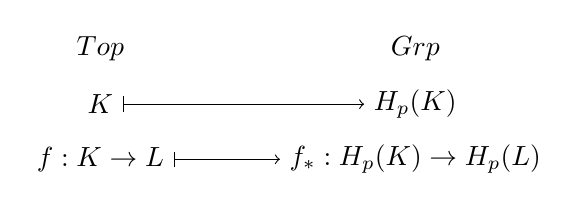
\begin{tikzpicture}
			\node (Top) at (0,0) {$ \category{Top} $};
			\node (Grp) at (4,0) {$ \category{Grp} $};
			\node (ObT) at (0,-0.7) {$ \abs{K} $};
			\node (ObG) at (4,-0.7) {$ H_p(K) $};
			\node (MorT) at (0,-1.4) {$ f : K\to L $};
			\node (MorG) at (4,-1.4) {$ f_* : H_p(K)\to H_p(L) $};
			\draw[|->] (ObT) -- (ObG);
			\draw[|->] (MorT) -- (MorG);
		\end{tikzpicture}
	\end{center}
	给出了一个从 $ \category{Top} $ 到 $ \category{Grp} $ 的函子.
\end{Theorem}
\begin{Proof}
	为此只需验证 $ \id : \abs{K}\to\abs{K} $ 被作用变成 $ \id_* : H_p(K)\to H_p(K) $, 和对 $ f : \abs{K}\to \abs{L} $, $ h : \abs{L}\to\abs{M} $, 有 $ (hf)_*=h_*f_* $.

	其中第一条是显然的, 这里只证明第二条. 考虑以下的交换图:
	\begin{center}
		\begin{tikzcd}
			\abs{K} \arrow[r, "f"]                     & \abs{L} \arrow[r, "h"]                  & \abs{M} \\
			K                                          & L                                       & M       \\
													   & L' \arrow[u, "g"] \arrow[ru, "\varphi"] &         \\
			K' \arrow[ru, "\varphi'"] \arrow[uu, "g'"] &                                         &        
		\end{tikzcd}
	\end{center}
	则 $ h_*=\varphi_*g_*^{-1} $, $ f_*=(g\varphi')_*(g_*')^{-1} $, 计算得到
	\[
		\begin{aligned}
			h_*f_*&=\varphi_*g_*^{-1}g_*\varphi'_*(g_*')^{-1}\\
			(hf)_*&=(\varphi\varphi')_*(g_*')^{-1}=\varphi_*\varphi_*'(g_*')^{-1}
		\end{aligned}
	\]
	也即 $ (hf)_*=h_*f_* $.\qed
\end{Proof}

\begin{Corollary}
	同调群是同胚不变量.
\end{Corollary}
\begin{Proof}
	对 $ \abs{K}\cong\abs{L} $, 考虑 $ f : C(\abs{K},\abs{L}) $, $ h\in C(\abs{L},\abs{K}) $ 使得 $ fh=\id_{\abs{L}} $, $ hf=\id_{\abs{K}} $. 由~\ref{thm:同调群函子}~可知
	\[
		f_*h_*=(fh)_*=(\id_{\abs{L}})_*=\id,\qquad h_*f_*=(hf)_*=(\id_{\abs{K}})_*=\id,
	\]
	也即 $ f_* $ 和 $ h_* $ 是同构, 得到 $ H_p(K)\cong H_p(L) $.\qed
\end{Proof}

我们知道:
\begin{center}
	\begin{tikzpicture}
		\node (Cong) at (0,0) {同胚 $ X\cong Y $};
		\node (Hopt) at (3,0) {同伦 $ X\simeq Y $};
		\node (CongI) at (0,-1) {同胚不变量};
		\node (HoptI) at (3,-1) {同伦不变量};
		\draw[-Implies, double equal sign distance] (Cong) -- (Hopt);
		\draw[-Implies, double equal sign distance] (HoptI) -- (CongI);
	\end{tikzpicture}
\end{center}
所以如果可以验证同调群是同伦不变量, 那么从逻辑上讲, 自然就不必说明它是同胚不变量. 幸运的是, 确实如此. 在这里只证明 $ K $ 是有限复形的情形:

\begin{Theorem}
	设 $ f,g\in C(\abs{K},\abs{L}) $, $ K $ 是有限复形. 若 $ f\simeq g $, 则 $ f_*=g_* $.
\end{Theorem}
\begin{Proof}
	因 $ K $ 是有限复形, $ H $ 是连接 $ f $ 与 $ g $ 的同伦, 故 $ \abs{K}\times I $ 是紧度量空间. 考虑 $ \abs{K}\times I $ 的开覆盖
	\[
		\CC=\set{H^{-1}(\St(w,L)) : w\in L^{(0)}},
	\]
	由 Lebesgue 覆盖引理可知
	\[
		\exists\delta>0\,\forall x\in\abs{K}\times I\,\exists w\in L^{(0)}\,(B(x,\delta)\subset H^{-1}(\St(w,L))).
	\]
	而存在 $ m\in\Zi $ 和 $ k>0 $ 使得 $ v\in(\sd^m\,K)^{(0)} $, 且
	\[
		\St(v,\sd^m\,K)\times\left[ \frac{r-1}{k},\frac{r}{k} \right]\subset B(x,\delta).
	\]
	也即存在 $ w\in L^{(0)} $ 使得
	\[
		\St(v,\sd^m\,K)\times\left[ \frac{r-1}{k},\frac{r}{k} \right]\subset H^{-1}(\St(w,L)).
	\]
	这导出
	\[
		h_{(r-1)/k}(\St(v,\sd^m\,K))\subset\St(w,L),\quad h_{r/k}(\St(v,\sd^m\,K))\subset\St(w,L).
	\]
	意味着 $ h_{(r-1)/k} $ 和 $ h_{r/k} $ 可以取到相同的单纯逼近 $ \varphi_r : \sd^m\,K\to L $. 而 $ \id : \sd^m\,K\to K $ 也有相应的单纯逼近, 于是
	\[
		\forall 1\leqslant r\leqslant k\,(h_{(r-1)/k})_*=(h_{r/k})_*,
	\]
	那么
	\[
		f_*=(h_0)_*=(h_{1/r})_*=\dots=(h_{(k-1)/k})_*=(h_1)_*=g_*.
	\]
	命题得证.\qed
\end{Proof}

\begin{Corollary}[同调群是同伦不变量]
	若 $ \abs{K}\simeq\abs{L} $, 则 $ H_p(\abs{K})\cong H_p(\abs{L}) $.
\end{Corollary}
\begin{Proof}
	这即存在 $ f\in C(\abs{K},\abs{L}) $, $ g\in C(\abs{L},\abs{K}) $ 使得
	\[
		fg\simeq\id_{\abs{L}},\qquad gf\simeq\id_{\abs{K}},
	\]
	由此 $ f_* $ 与 $ g_* $ 互逆. 即 $ H_p(\abs{K})\cong H_p(\abs{L}) $.\qed
\end{Proof}

\subsection{应用: 映射度, Brouwer 不动点定理}

考虑到 $ \S^0 $ 退化, 不妨总假设 $ n>0 $. Brouwer 不动点主要讨论球面上的映射:

\begin{Definition}[映射度]
	设 $ f\in C(\S^n,\S^n) $, 它诱导
	\[
		f_* : H_n(\S^n)\to H_n(\S^n),\quad \alpha\mapsto f_*(\alpha)=d\alpha, d\in\Z.
	\]
	其中 $ \alpha $ 是 $ \S^n $ 的生成元. $ d $ 称作 $ f $ 的\emph{映射度}, 记作 $ \deg f $.
\end{Definition}

当 $ n=1 $ 时, 映射度 $ \deg f $ 有明显的几何意义. $ \deg f $ 即 $ f $ 覆盖球面的层数. $ \pi_1(\S^1)=[\S^1,\S^1]\to\Z $, $ f\mapsto\deg f $ 给出了 $ \S^1 $ 的基本群.

\begin{Proposition}\label{prop:映射度的基本性质}
	映射度具有以下基本性质: 以下设 $ f,g : \S^n\to\S^n $,
	\begin{enumerate}
		\item 若 $ f\simeq g $, 则 $ \deg f=\deg g $;
		\item $ \deg(gf)=\deg f\cdot\deg g $;
		\item $ \deg\id=1 $. 若 $ c $ 是常值映射, 则 $ \deg c=0 $.
	\end{enumerate}
\end{Proposition}
\begin{Proof}
	(2) 因
	\[
		\deg(gf)\alpha=(gf)_*\alpha=g_*(\deg f\alpha)=\deg f\cdot g_*\alpha=\deg f\cdot\deg g\alpha.
	\]
	而 (1), (3) 是显然的.\qed
\end{Proof}

\begin{Lemma}\label{lem:边缘限制映射度为0}
	设 $ F\in C(\D^{n+1},\S^n) $, 则 $ \deg(F|_{\partial\D^{n+1}})=0 $.
\end{Lemma}
\begin{Proof}
	这因
	\begin{center}
		\begin{tikzcd}
			\S^n \arrow[r, "\iota", hook]        & \D^{n+1} \arrow[r, "F"]        & \S^n      \\
			H_n(\S^n) \arrow[r, "\iota_*", hook] & H_n(\D^{n+1}) \arrow[r, "F_*"] & H_n(\S^n)
		\end{tikzcd}
	\end{center}
	且 $ F|_{\partial\D^{n+1}}=F\circ\iota $. 由 $ H_n(\D^{n+1})=0 $ 可知 $ (F|_{\partial\D^{n+1}})_*=0 $.\qed
\end{Proof}

\begin{Lemma}
	不存在这样的 $ r\in C(\D^{n+1},\S^n) $ 使得 $ r|_{\partial \D^{n+1}}=\id_{\S^n} $.
\end{Lemma}
\begin{Proof}
	由~\ref{lem:边缘限制映射度为0}~可知若存在这样的 $ r $, 有 $ \deg(r|_{\partial\D^{n+1}})=0 $. 再由~\ref{prop:映射度的基本性质}~可知 $ \deg(\id_{\S^n})=1 $, 矛盾.\qed
\end{Proof}

\begin{Theorem}[Brouwer 不动点的定理]\label{thm:Brouwer 不动点定理}
任何的 $ f\in C(\D^n,\D^n) $ 存在不动点.
\end{Theorem}
\begin{Proof}
	用反证法, 任取 $ x\in\D^n $, 都有 $ f(x)\ne x $. 取
	\[
		h : \D^n\to\S^{n+1},\qquad x\mapsto\frac{x-f(x)}{\norm{x-f(x)}}.
	\]
	由~\ref{lem:边缘限制映射度为0}~可知 $ \deg(h|_{\partial\D^n})=0 $, 作同伦
	\[
		H : \S^{n-1}\times I\to\S^{n-1},\qquad (x,t)\mapsto\frac{x-tf(x)}{\norm{x-tf(x)}}.
	\]
	这一同伦的定义是合理的, 因 $ x\ne f(x) $ 可知 $ t=1 $ 时 $ x-f(x)\ne 0 $, 而 $ 0\leqslant t<1 $ 时若有 $ x=tf(x) $, 则
	\[
		1=\norm{x}=\norm{tf(x)}=t\norm{f(x)}\leqslant t<1
	\]
	矛盾. 此时
	\[
		H(x,0)=\id_{\S^{n-1}}(x),\qquad H(x,1)=h|_{\partial\D^n}(x),
	\]
	即 $ \id_{\S^{n-1}}\simeq h|_{\partial\D^n} $, 而它们的映射度不相等, 矛盾.\qed
\end{Proof}

Brouwer 不动点定理在 $ n=1 $ 时即为介值定理, 在 $ n=2 $ 时使用分析的方法已经比较繁琐, 但还是可以借助基本群来解决. 以上给出了 $ n\geqslant 1 $ 时使用同调论的解决方法.

接下来考虑从球面到球面的映射, $ f\in C(\S^n,\S^n) $ 可以不存在任何不动点, 最常见的取法就是取\emph{对径映射} $ r : x\mapsto -x $.

\begin{Proposition}
	$ \deg r=(-1)^{n+1} $.
\end{Proposition}
\begin{Proof}
	考虑 $ r_i : \S^n\to\S^n $, 它只将第 $ i $ 个分量反转, 即
	\[
		(x_1,\dots,x_i,\dots,x_{n+1})\mapsto (x_1,\dots,-x_i,\dots,x_{n+1}).
	\]
	则 $ r=r_{n+1}r_n\cdots r_1 $. 于是 $ \deg r=\prod_{i=1}^{n+1}\deg r_i $. 由
	\begin{center}
		\begin{tikzcd}
			{(x_1,\dots,x_i,\dots,x_{n+1})} \arrow[d, maps to] & \S^n \arrow[r, "r_i"] \arrow[d, "{h_{i,n+1}}"] & \S^n \arrow[d, "{h_{i,n+1}}"] & {(x_1,\dots,-x_i,\dots,x_{n+1})} \arrow[d, maps to] \\
			{(x_1,\dots,x_{n+1},\dots,x_i)}                    & \S^n \arrow[r, "r_{n+1}"]                      & \S^n                          & {(x_1,\dots,-x_{n+1},\dots,x_i)}                   
		\end{tikzcd}
	\end{center}
	有 $ r_{n+1}=h_{i,n+1}r_ih_{i,n+1}^{-1} $, 从而
	\[
		\deg r_{n+1}=\deg h_{i,n+1}\deg r_i\deg h_{i,n+1}^{-1}=\deg r_i.
	\]
	故 $ \deg r=(\deg r_{n+1})^{n+1} $.

	考虑 $ \S^n $ 的如下三角剖分:
	\begin{figure}[htbp]
		\centering
		\includegraphics[width=0.25\linewidth]{figures/Sec7-1.png}
	\end{figure}
	它由 $ \R^{n+1} $ 上典范正交基的顶点 $ \set{\pm e_1,\pm e_2,\dots,\pm e_{n+1}} $ 确定. 记 $ e_{-i}=-e_i $, 得到复形 $ K $
	\[
		\abs{K}=\set{(x_1,\dots,x_{n+1})\in\R^{n+1} : \sum_{i=1}^{n+1}\abs{x_i}=1}.
	\]
	考虑中心辐射 $ \varphi : \abs{K}\to\S^n $, 有
	\begin{center}
		\begin{tikzcd}
			\S^n \arrow[r, "r_{n+1}"]                                 & \S^n                          \\
			\abs{K} \arrow[r, "\tilde r_{n+1}"] \arrow[u, "\varphi"'] & \abs{K} \arrow[u, "\varphi"'] \\
			{(x_1,\dots,x_n,x_{n+1})} \arrow[r, maps to]              & {(x_1,\dots,x_n,-x_{n+1}}    
		\end{tikzcd}
	\end{center}
	那么对 $ K $ 中的 $ n $ 维单形, 给定如下的定向: (\textit{约定 $ i_j=\pm j $})
	\[
		\pm[e_{i_1},e_{i_2},\dots,e_{i_{n+1}}]\begin{cases}
			\text{取}+\Longleftrightarrow \set{i_k}\,\text{中有偶数个负数}\\\text{取}-\Longleftrightarrow \set{i_k}\,\text{中有奇数个负数}
		\end{cases}
	\]
	令 $ z_n=\sum_{\sigma\in\S^n_+(K)}\sigma $ 可知 $ \partial z_n=0 $. 这里 $ \S^n_+(K) $ 是 $ K $ 中正定向 $ n $ 维单形全体. 此时 $ z_n\in Z_n(K)=H_n(\S^n) $, 那么
	\[
		(\tilde{r}_{n+1})_\sharp : C_n(K)\to C_n(K),\qquad \pm[e_1,\dots,e_{n+1}]\mapsto\mp[e_1,\dots,e_{n+1}].
	\]
	故 $ (\tilde{r}_{n+1})\sharp(z_n)=-z_n $, 由此 $ \deg\tilde{r}_{n+1}=-1 $ 得到 $ \deg r_{n+1}=-1 $.\qed
\end{Proof}

\begin{Proposition}\label{prop:球面不动点}
	设 $ h\in C(\S^n,\S^n) $, 若 $ \deg h\ne(-1)^{n+1} $, 则 $ h $ 必有不动点.
\end{Proposition}
\begin{Proof}
	用反证法, 设 $ \forall x\in\S^n\,(h(x)\ne x) $. 取
	\[
		H : \S^n\times I\to\S^n,\qquad (x,t)\mapsto\frac{(1-t)h(x)+t(-x)}{\norm{(1-t)h(x)+t(-x)}}.
	\]
	类似地, 若有 $ (1-t)h(x)-tx=0 $, 则
	\[
		\norm{(1-t)h(x)}=t\norm{x}\Longrightarrow 1-t=t\Longrightarrow t=\frac{1}{2}.
	\]
	而将 $ t=1/2 $ 代入之后有 $ 1/2(h(x)-x)\ne 0 $, 于是 $ H $ 是合理定义的. 此时由
	\[
		H(x,0)=h(x),\qquad H(x,1)=r(x)
	\]
	可知 $ h\simeq r $, 而 $ \deg h\ne\deg r=(-1)^{n+1} $, 矛盾.\qed
\end{Proof}

\begin{Corollary}\label{cor:对径点的存在性}
	取 $ f\in C(\S^n,\S^n) $, $ \deg f\ne 1 $, 则存在 $ x_0\in\S^n $ 使得 $ f(x_0)=-x_0 $.
\end{Corollary}
\begin{Proof}
	考虑 $ rf : \S^n\to\S^n $, 有 $ \deg(rf)\ne(-1)^{n+1} $. 由~\ref{prop:球面不动点}~可知 $ rf $ 存在不动点 $ x_0 $, 那么
	\[
		rf(x_0)=x_0\Longrightarrow -f(x_0)=x_0,
	\]
	于是命题得证.\qed
\end{Proof}

下面把这一问题应用于所谓的 ``毛球问题'':

\begin{Definition}[向量场]
	称 $ v : X\to\R^n $ 是一个 $ X $ 上的\emph{向量场}(当 $ n=1 $ 时称为\emph{数量场}). 特别地, $ v : \S^n\to\R^{n+1} $ 称作一个切向量场, 若对任意 $ x\in\S^n $ 都有 $ \lrangle{x,v(x)}=0 $.
\end{Definition}

\begin{Corollary}[Brouwer--Poincar\'e]\label{cor:毛球定理}
	$ \S^n $ 上存在非零切向量场(\textit{向量场非零指它在任何一点都非零.})当且仅当 $ n $ 为奇数.
\end{Corollary}
\begin{Proof}
	\textit{充分性.} 因 $ n=2k-1 $, 直接取
	\[
		v : \S^n\to\S^n,\qquad (x_1,x_2,\dots,x_{2k-1},x_{2k})\mapsto(-x_2,x_1,\dots,-x_{2k},x_{2k-1})
	\]
	是一个非零切向量场即可.

	\textit{必要性.} 若 $ \S^n $ 存在非零切向量场 $ v $, 考虑它诱导的映射
	\[
		h : \S^n\to\S^n,\qquad x\mapsto\frac{v(x)}{\norm{v(x)}},
	\]
	因 $ v $ 是切向量场, 故 $ h $ 也是切向量场, 于是
	\[
		\forall x\in\S^n\,(h(x)\ne x\land h(x)=-x).
	\]
	由~\ref{prop:球面不动点}~可知 $ \deg h=(-1)^{n+1} $, 又由~\ref{cor:对径点的存在性}~可知 $ \deg h=1 $, 于是 $ n $ 是奇数.\qed
\end{Proof}

\subsection{应用: Euler 示性数, Lefschetz 不动点定理}

设 $ K $ 是有限复形, 但 $ H_p(K)=\ker\partial_p/\im\partial_{p+1} $ 未必是自由的, 但一定是有限生成 Abel 群. 而有限生成 Abel 群 $ G $ 总有分解
	\[
		G\cong\Z\oplus\Z\oplus\dots\oplus\Z\oplus(\Z/t_1\Z)\oplus(\Z/t_2\Z)\oplus\dots\oplus(\Z/t_k\Z)=F(G)\oplus T(G),
	\]
	其中 $ F(G) $ 是 $ G $ 的自由部分, 它有秩 $ r $, $ T(G) $ 是 $ G $ 的挠部分, 满足 $ t_1\mid t_2\mid\dots\mid t_k $, 则 $ H_i(K) $ 中自由部分的秩 $ \beta_1(K):=\rank F(H_i(K)) $ 称作复形 $ K $ 的第 $ i $ 个 \emph{Betti 数}.

	我们把 Brouwer 定理再次推广, 不仅仅考虑球面之间的映射, 而考虑一般的复形 $ K $, 它的几何实现到自身的映射 $ f\in C(\abs{K},\abs{K}) $ 的不动点. 为此, 我们先回顾一点点初等线性代数的内容:

\begin{Definition}[线性变换的迹]
	设 $ \varphi : V\to V $ 是线性变换 $ \set{e_1,\dots,e_n} $ 是 $ V $ 的基, $ \varphi $ 在 $ \set{e_i} $ 下的矩阵为 $ A $. 因迹对基变换是不变的, 于是可以定义
	\[
		\tr\varphi:=\tr A
	\]
	是线性变换 $ \varphi $ 的\emph{迹}.
\end{Definition}

\begin{Lemma}\label{lem:分解引理}
	设 $ W $ 是 $ V $ 的 $ \varphi $--不变子空间, 即 $ \varphi(W)\subset W $, 则 $ \varphi $ 可以诱导
	\[
		\varphi_* : V/W\to V/W,\qquad x+W\mapsto \varphi(x)+W,
	\]
	此时有
	\[
		\tr\varphi=\tr(\varphi|_W)+\tr\varphi_*.
	\]
\end{Lemma}
\begin{Proof}
	设 $ W $ 有一组基 $ \set{\xi_1,\dots,\xi_r} $, $ V $ 的基 $ \set{\xi_1,\dots,\xi_r,\xi_{r+1},\dots,\xi_n} $ 由 $ W $ 的基扩张而来, 则 $ V/W $ 以 $ \set{\xi_{r+1}+W,\dots,\xi_n+W} $ 为一组基. 设 $ \varphi|_W $, $ \varphi $ 和 $ \varphi_* $ 在对应基下的矩阵分别为 $ A, A_W, A_* $, 则
	\[
		A=\mqty[A_w & * \\ ~ & A_*],
	\]
	这导出 $ \tr\varphi=\tr(\varphi|_W)+\tr\varphi_* $.\qed
\end{Proof}

设 $ G $ 是有限生成的自由 Abel 群, $ \varphi : G\to G $ 是线性映射. 也可以定义 $ \tr\varphi $: 考虑 $ G $ 的 $ \varphi $--不变子群 $ H $, 那么 $ \varphi $ 可以诱导商群上的线性映射
\[
	\varphi_* : G/H\to G/H,
\]
当 $ G/H $ 也是自由群时, 仍然有 $ \tr\varphi=\tr(\varphi|_H)+\tr\varphi_* $.

为了记号方便, 我们约定将链群、闭链群、边缘链群中的复形记号省略掉, 并且记
\[
	H_p=Z_p/B_p=T_p\oplus F_p,
\]
这里 $ T_p $ 是 $ H_p $ 的挠部分, $ F_p $ 是 $ H_p $ 的自由部分. 那么 $ Z_p $ 可以分解成两部分, 一部分被 $ B_p $ 抹掉之后产生挠部分, 把这一部分记作
\[
	W_p:=\set{c_p\in C_p : \exists \ell\in\Z\sm\set{0}\,(\ell c_p\in B_p)}.
\]
另一部分被 $ B_p $ 模掉产生自由部分.

\begin{Theorem}[Hopf 迹定理]
	设 $ \varphi : \CC(K)\to\CC(K) $ 是链映射, $ K $ 是有限复形, 那么
	\[
		\sum_{p}(-1)^p\tr\varphi|_{C_p}=\sum_{p}(-1)^p\tr(\varphi_*, H_p/T_p),
	\]
	这里 $ \varphi_* $ 是合理定义的. (\textit{因形如 $ \Z/m\Z\to\Z $ 的同态必为零同态, 于是一定 $ \varphi(T_p)\leqslant T_p $.})
\end{Theorem}
\begin{Proof}
	根据前面约定的记号, 容易得到
	\[
		B_p\leqslant W_p\leqslant Z_p\leqslant C_p.
	\]

	首先考虑 $ Z_p\leqslant C_p $. 由 $ C_p\stackrel{\partial_p}{\twoheadrightarrow}B_{p-1}\leqslant C_{p-1} $ 且 $ Z_p=\ker\partial_p $, 由第一同构定理得到
	\[
		C_p/Z_p\cong B_{p-1}.
	\]
	因 $ B_{p-1} $ 自由, 故 $ C_p/Z_p $ 自由. 由~\ref{lem:分解引理}~可知
	\[
		\tr(\varphi|_{C_p})=\tr(\varphi|_{Z_p})+\tr(\varphi_*,C_p/Z_p)=\tr(\varphi|_{Z_p})+\tr(\varphi_*,B_{p-1}).
	\]

	再考虑 $ W_p\leqslant Z_p $. 由
	\begin{center}
		\begin{tikzcd}
			Z_p \arrow[r, "\pi_{B_p}", two heads] \arrow[rr, "j", bend left] & H_p \arrow[r, "\pi_{T_p}", two heads]           & F_p           \\
			z_p \arrow[r, maps to]                                           & \set{z_p}=z_p+B_p \arrow[r, maps to] & \set{z_p}+T_p
		\end{tikzcd}
	\end{center}
	则对任何 $ z_p\in W_p $, 有 $ j(z_p)=\set{z_p}+T_p $. 由 $ W_p $ 的定义可知存在 $ \ell\in\Z\sm\set{0} $ 使得 $ \ell z_p\in B_p $. 那么
	\[
		\ell\set{z_p}+T_p=\set{\ell z_p}+T_p=0+T_p,
	\]
	即 $ W_p\leqslant\ker j $. 反之, 任取 $ z_p\in\ker j $, 由
	\[
		j(z_p)=\set{z_p}+T_p=0\Longrightarrow\exists\ell\in\Z\sm\set{0}\,(\ell\set{z_p}=0)\Longrightarrow z_p\in W_p
	\]
	知 $ \ker j\subset W_p $. 于是 $ W_p=\ker j $, 由第一同构定理可知
	\[
		Z_p/W_p\cong H_p/T_p=F_p.
	\]
	由 $ F_p $ 自由可知 $ Z_p/W_p $ 也自由, 由~\ref{lem:分解引理}~可知
	\[
		\tr(\varphi|_{Z_p})=\tr(\varphi|_{W_p})+\tr(\varphi_*,Z_p/W_p)=\tr(\varphi|_{W_p})+\tr(\varphi_*,F_p).
	\]

	最后, 考虑 $ B_p\leqslant W_p $. 我们断言 $ \rank B_p=\rank W_p $ 且 $ \tr(\varphi|_{B_p})=\tr(\varphi|_{W_p}) $. 用反证法, 否则 $ m=\rank B_p<\rank W_p=r $.

	设 $ \set{\alpha_1,\dots,\alpha_r} $ 是 $ W_p $ 的一组基, 不妨设 $ n_i\in\Zi $, $ \set{n_1\alpha_1,\dots,n_m\alpha_m} $ 是 $ B_p $ 的一组基. 那么由 $ r>m $ 可知存在 $ n_{m+1}\in\Zi $ 使得 $ n_{m+1}\alpha_{m+1}\in B_p $(\textit{这由 $ W_p $ 的定义可得}), 矛盾, 于是 $ r=m $.

	设 $ \varphi|_{W_p} $ 在 $ \set{\alpha_1,\dots,\alpha_r} $ 下的矩阵为 $ A=[a_{ij}] $, $ \varphi|_{B_p} $ 在 $ \set{n_1\alpha_1,\dots,n_r\alpha_r} $ 下的矩阵为 $ B=[b_{ij}] $. 则
	\[
		\varphi|_{W_p}(\alpha_j)=\sum_{i=1}^ra_{ij}\alpha_i\Longrightarrow\varphi|_{W_p}(n_j\alpha_j)=\sum_{i=1}^ra_{ij}n_j\alpha_i.
	\]
	且
	\[
		\varphi|_{B_p}(n_j\alpha_j)=\sum_{i=1}^rb_{ij}n_i\alpha_i.
	\]
	而 $ B_p\leqslant W_p $, 于是 $ \sum_{i=1}^ra_{ij}n_j\alpha_i=\sum_{i=1}^rb_{ij}n_i\alpha_i $, 这说明对任意 $ i,j $ 成立
	\[
		a_{ij}n_j=b_{ij}n_i.
	\]
	特别地, 当 $ i=j $ 时就有 $ a_{ii}=b_{ii} $. 那么
	\[
		\tr(\varphi|_{W_p})=\tr A=\sum_{i=1}^ra_{ii}=\sum_{i=1}^rb_{ii}=\tr B=\tr(\varphi|_{B_p}).
	\]

	于是:
	\[
		\begin{aligned}
			\tr(\varphi|_{C_p})&=\tr(\varphi|_{Z_p})+\tr(\varphi|_{B_{p-1}})\\
			&=\tr(\varphi|_{W_p})+\tr(\varphi_*,F_p)+\tr(\varphi|_{B_{p-1}})\\
			&=\tr(\varphi|_{B_p})+\tr(\varphi|_{B_{p-1}})+\tr(\varphi_*,F_p).
		\end{aligned}
	\]
	因 $ K $ 是有限复形, 于是下面的交错和是有限和, 得到
	\[
		\begin{aligned}
			\sum_{p\geqslant 0}(-1)^p\tr(\varphi|_{C_p})&=\sum_{p\geqslant 0}(-1)^p\tr(\varphi|_{B_p})-(-1)^{p-1}\tr(\varphi|_{B_{p-1}})+(-1)^p\tr(\varphi_*,F_p)\\
			&=\sum_{p\geqslant 0}(-1)^p\tr(\varphi_*,F_p).
		\end{aligned}
	\]
	于是定理成立.\qed
\end{Proof}

我们再进一步讨论一下这些子群: 由 $ Z_p/W_p\cong H_p/T_p $, 若记 $ Z_p=W_p\oplus A $, 那么由 $ W_p/B_p\cong T_p $,
\[
	\frac{Z_p}{B_p}\cong\frac{W_p\oplus A}{B_p}\cong\frac{W_p}{B_p}\oplus\frac{A}{B_p}\cong T_p\oplus A,
\]
这说明 $ A\cong F_p $.

\begin{Definition}[Lefschetz 数]
	设 $ K $ 是有限复形, $ h : \abs{K}\to\abs{K} $ 是连续映射, 称
	\[
		\Lambda(h):=\sum_{p}(-1)^p\tr(h_*,H_p/T_p)
	\]
	是 $ h $ 的 \emph{Lefschetz 数}.
\end{Definition}

由定义可知若 $ h\simeq h' $, 则 $ \Lambda(h)=\Lambda(h') $, 这因 $ h_*=h_*' $; 同时 $ \Lambda(h) $ 与 $ \abs{K} $ 的三角剖分无关, 因为之前已经说明过同调群不会随着重分改变. 

特别地, 若允许同调群中的系数在数域中取值, 那么 $ C_p $ 和 $ H_p $ 都是向量空间, 其维数即为复形 $ K $ 的 $ p $ 阶 Betti 数, 也即 $ \dim_\F H_p=\beta_p(K) $.

考虑 $ \id : \abs{K}\to\abs{K} $ 的 Lefschetz 数:
\[
	\Lambda(\id)=\sum_{p\geqslant 0}(-1)^p\tr(\id_*,H_p/T_p)=\sum_{p\geqslant 0}(-1)^p\beta_p(K).
\]
设 $ K $ 的 $ p $ 维单形个数为 $ f_p $, 取 $ f(K)=(f_0,\dots,f_n) $, 那么
\[
	\rank C_p(K)=f_p=\beta_p(K).
\]
称
\[
	\chi(K)=\sum_{p\geqslant 0}(-1)^p\rank C_p(K)
\]
是 $ K $ 的 \emph{Euler 示性数}.

\begin{Theorem}[Euler--Poincar\'e]
	Euler 示性数是拓扑不变量, 它与 $ \abs{K} $ 的三角剖分无关, 且
	\[
		\chi(\abs{K})=\sum_{p\geqslant 0}(-1)^p\beta_p(K).
	\]
\end{Theorem}

一些典型的曲面 Euler 示性数可以计算出来:
\[
	\chi(\T^2)=0,\quad \chi(S)=0,\quad \chi(\mathbb{RP}^2)=1,\quad \chi(\S^n)=\begin{cases}
		2, & n=2k \\ 0, & n=2k+1
	\end{cases}.
\]

\begin{Theorem}[Lefschetz 不动点定理]\label{thm:Lefschetz 不动点定理}
	设 $ K $ 是有限复形, $ h\in C(\abs{K},\abs{K}) $, 若 $ \Lambda(h)\ne 0 $, 则 $ h $ 必有不动点.
\end{Theorem}
\begin{Proof}
	用反证法, 设 $ \forall x\in\abs{K}\,(h(x)\ne x) $, 考虑连续函数
	\[
		f : \abs{K}\to\R,\qquad x\mapsto\norm{x-h(x)},
	\]
	因 $ \abs{K} $ 是紧度量空间, 它取到最小值 $ \varepsilon $. 不妨设 $ \mesh K<\varepsilon/2 $ (\textit{否则取足够多次数的标准重心重分}).

	记 $ h : \abs{K}\to\abs{K} $ 得单纯逼近为 $ \varphi : \sd^m\,K\to K $, 则对任意 $ x\in K $, $ h(x) $ 和 $ \varphi(x) $ 都落在 $ K $ 的同一个单形中, 有
	\[
		\norm{h(x)-\varphi(x)}\leqslant\mesh K<\frac{\varepsilon}{2},
	\]
	故
	\[
		\norm{x-\varphi(x)}\geqslant\norm{x-h(x)}-\norm{h(x)-\varphi(x)}>\frac{\varepsilon}{2}.
	\]

	由代数重分定理:
	\begin{center}
		\begin{tikzcd}
			C_p(K) \arrow[r, "\exists!\lambda"] \arrow[rr, "\xi_p", bend left] & {C_p(\sd^m\,K)} \arrow[r, "\varphi_\sharp"] & C_p(K)
		\end{tikzcd}
	\end{center}
	则 $ h_*=(\varphi_\sharp\lambda)_*=\xi_* $. 故
	\[
		\Lambda(h)=\sum_{p\geqslant 0}(-1)^p\tr(h_* : H_p/T_p)=\sum_{p\geqslant 0}(-1)^p\tr(\xi_*, C_p).
	\]
	我们断言 $ \tr(\xi_*, C_p)=0 $. 这蕴含着 $ \xi_p $ 在 $ S_p^+(K) $ (\textit{ $ K $ 的定向 $ p $ 维单形全体, 这是 $ C_p(K) $ 的一组基}) 下的矩阵 $ A $ 满足 $ \tr A=0 $. 这意味着 $ \xi_p(\sigma) $ 中不能含有 $ \sigma $. 因 $ \lambda(\sigma) $ 被 $ \sd^m\,K_\sigma $ 承载, 若
	\[
		\xi_p(\sigma)=\varphi_\sharp\lambda(\sigma)=a\sigma+\cdots,\quad a\ne 0,
	\]
	在 $ \lambda(\sigma) $ 的展开式中应当存在 $ p $ 维单形 $ \tau\in\sd^m\,K_\sigma $ 使得
	\[
		\varphi_\sharp(\tau)=a'\sigma+\cdots,\quad a'\ne 0.
	\]
	因对任意 $ x\in\tau $ 都有 $ \varphi(x)\in\sigma $, 又 $ \tau\subset\sigma $, 故 $ x\in\sigma $, 从而
	\[
		\frac{\varepsilon}{2}<\norm{x-\varphi(x)}\leqslant\mesh K<\frac{\varepsilon}{2},
	\]
	矛盾.\qed
\end{Proof}

\begin{Corollary}
	$ \S^n $ 上的对径映射满足 $ \deg r=(-1)^{n+1} $.
\end{Corollary}
\begin{Proof}
	由~\ref{thm:Lefschetz 不动点定理}~知 $ \Lambda(r)=1+(-1)^n\deg r=0 $.\qed
\end{Proof}

\begin{Corollary}
	设 $ K $ 是零调的, 则任意 $ f\in C(\abs{K},\abs{K}) $ 都存在不动点.
\end{Corollary}
\begin{Proof}
	设 $ f_* : H_0(K)\to H_0(K) $, 它有单纯逼近 $ \varphi : K'\to K $, 那么图
	\begin{center}
		\begin{tikzcd}
			C_0(K) \arrow[rd, "\varepsilon"] \arrow[rr, "\lambda"] &    & C_0(K') \arrow[ld, "\varepsilon'"] \arrow[r, "\varphi_\sharp"] & C_0(K) \\
																   & \Z &                                                                &       
		\end{tikzcd}
	\end{center}
	交换.

	对 $ v\in K^{(0)} $, $ K_v'=\set{v} $, 有 $ \lambda(v)=\ell v $. 由
	\[
		1=\varepsilon(v)=\varepsilon'\lambda(v)=\ell\varepsilon'(v)=\ell
	\]
	可知 $ \lambda(v)=v $, 于是
	\[
		\varphi_\sharp(\lambda(v))=\varphi_\sharp(v)=\varphi(v)
	\]
	与 $ v $ 在同一同调类中, 这即 $ f_*(\set{v})=\set{\varphi_*(\lambda(v))}=\set{v} $, 即 $ f_*=\id_* $. 故 $ \Lambda(f)=\Lambda(\id)=1\ne 0 $. 由~\ref{thm:Lefschetz 不动点定理}~得证.\qed
\end{Proof}

\begin{Corollary}
	设 $ \chi(\abs{K})=0 $, 则对任意同伦于 $ \id_{\abs{K}} $ 的连续映射 $ f\in C(\abs{K},\abs{K}) $, $ f $ 存在不动点.
\end{Corollary}
\begin{Proof}
	因 $ \Lambda(f)=\Lambda(\id)=\chi(\abs{K})\ne 0 $.\qed
\end{Proof}